\documentclass[class=article,border=5pt,tikz]{standalone}
\usepackage{pgfplots}
\pgfplotsset{compat=newest}
%\pgfplotsset{every non boxed x axis/.append style={x axis line style=-},
%     every non boxed y axis/.append style={y axis line style=-}}

\begin{document}
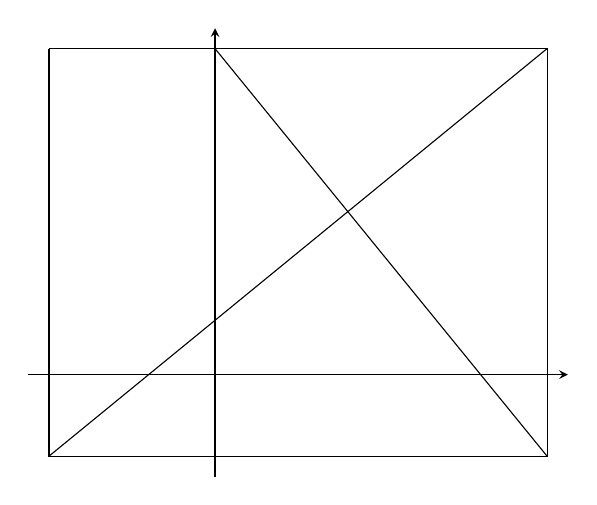
\begin{tikzpicture}[font=\tiny]
  \begin{axis}[
    axis lines = middle,
    xtick = \empty,
    ytick = \empty,
    xmin = -4.5,
    xmax = 8.5,
    ymin = -2.5,
    ymax = 8.5]
    \addplot[domain = 0:8] {8-(5/4)*x};
    \addplot[domain = -4:8] {4/3+(5/6)*x};
    \draw(axis cs:-4,8) -- (axis cs:8,8) -- (axis cs:8,-2) -- (axis cs:-4,-2) -- (axis cs:-4,8);
  \end{axis}
\end{tikzpicture}

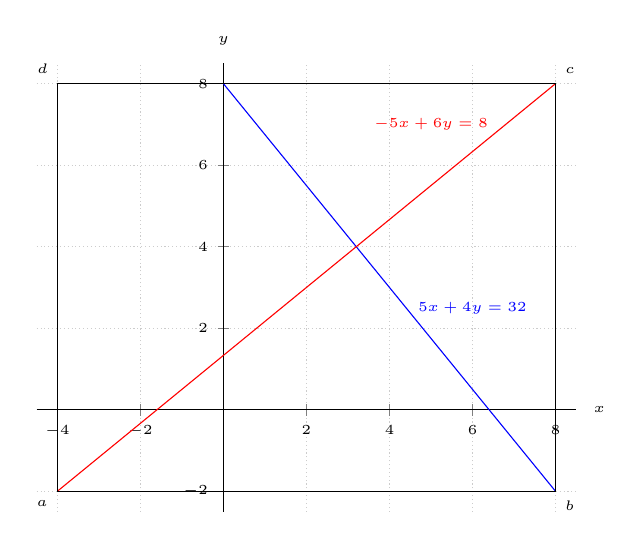
\begin{tikzpicture}[font=\tiny]
  \begin{axis}[
    axis lines = middle,
    x axis line style={-},
    y axis line style={-},
    x label style={at={(current axis.right of origin)},anchor=north,right=1mm},
    y label style={at={(current axis.above origin)},anchor=east,above=1mm},
    xlabel = {$x$},
    ylabel = {$y$},
    xmin = -4.5,
    xmax = 8.5,
    ymin = -2.5,
    ymax = 8.5,
    clip = false,
    grid = major,
    grid style = {densely dotted,black!20}]
    \node[below left] at (-4,-2) {$a$};
    \node[below right] at (+8,-2) {$b$};
    \node[above right] at (+8,+8) {$c$};
    \node[above left] at (-4,+8) {$d$};
    \addplot[blue,domain = 0:8] {8-(5/4)*x} 
        node at (6,2.5) {$5x+4y=32$};
    \addplot[red,domain = -4:8] {4/3+(5/6)*x} 
        node at (5,7) {$-5x+6y=8$};
    
    \draw(axis cs:-4,8) -- (axis cs:8,8) -- (axis cs:8,-2) -- (axis cs:-4,-2) -- (axis cs:-4,8);
  \end{axis}
\end{tikzpicture}
\end{document}


